\chapter{Estado del arte}

\section{Accesibilidad}

La "Guía de accesibilidad de aplicaciones móviles" (\cite{talero2020accesibilidadapps}) ofrece pautas esenciales para el desarrollo y evaluación de apps accesibles, dirigidas a personas con discapacidades. La guía se basa en la Directiva (UE) 2016/2102 y el Real Decreto 1112/2018, los cuales exigen la accesibilidad de aplicaciones en el sector público a partir de 2021.

Algunos puntos clave incluyen:

\begin{enumerate}
	\item Dificultades que enfrentan personas con discapacidades sensoriales, motrices y cognitivas, destacando la necesidad de adaptar las aplicaciones para estos perfiles de usuarios.

	\item Principios de desarrollo accesible, enfatiza la importancia de integrar la accesibilidad desde las primeras etapas del diseño y desarrollo, usando las herramientas de accesibilidad de los sistemas operativos.

	\item Se detallan directrices sobre cómo hacer que las interfaces de usuario sean accesibles, incluyendo la configuración del contraste, la visibilidad del foco y el tamaño de los componentes interactivos.

	\item La guía ofrece pautas para validar la accesibilidad de las aplicaciones mediante herramientas automáticas y manuales.

	\item Proporciona una lista de herramientas y productos de apoyo para facilitar la interacción de personas con discapacidades, como lectores de pantalla y magnificadores.
\end{enumerate}

En resumen, la guía ayuda a los desarrolladores a crear aplicaciones móviles que sean accesibles a todos los usuarios, mejorando la inclusión social y cumpliendo con los requisitos legales de accesibilidad.

\section{Dominio del problema}
Para comenzar, es necesario hablar un poco sobre conceptos generales en el mundo del deporte, definiendo algunos conceptos.

Un \textbf{ejercicio} es la repetición de un movimiento varias veces para estimular uno o varios músculos. Las \textbf{rutinas}, entendámolos como la colección de distintos ejercicios destinados a entrenar una parte o varias del cuerpo, a las rutinas también se les llama \textbf{entrenamientos}, pero en la app se referirá a rutinas como la anterior definición y los entrenamientos serán el hecho de haber realizado una rutina. Ejemplo, el entrenamiento del día 6 es hacer la rutina de flexiones. Una \textbf{serie} es cuando dentro de un ejercicio repetimos ese movimiento un número determinado de veces. Entre series se hacen descansos. Una \textbf{repetición}, es la realización del movimiento de ese ejercicio en una serie, es decir, si por ejemplo se están haciendo flexiones, se hacen 12, descanso, se hacen 10, descanso, se hacen 9 y ya no se hacen más flexiones, dentro del entrenamiento se vería así:

\underline {Rutina de entrenamiento 1:}
\begin{itemize}
	\item Ejercicio 1
	\begin{itemize}
		\item Serie 1: X repeticiones
		\item Descanso
		\item Serie 2: X repeticiones
	\end{itemize}
	\item Flexiones
	\begin{itemize}
		\item Serie 1: 12 repeticiones
		\item Descanso
		\item Serie 2: 10 repeticiones 
		\item Descanso
		\item Serie 3: 9 repeticiones
	\end{itemize}
	\item Ejercicio 3
	\begin{itemize}
		\item Serie 1: X repeticiones
		\item Descanso
		\item Serie 2: X repeticiones
	\end{itemize}
\end{itemize}

Las metas son objetivos que se pone el usuario en un ejercicio, por ejemplo, si un usuario desea llegar a hacer 10 flexiones mínimo en una serie la proxima vez que entrene, es que se ha puesto una meta de 10 flexiones.

El compartir una rutina es publicar los detalles de una rutina para que otra persona la pueda hacer en sus entrenamientos.

En este gremio del deporte es muy importante la planificación, ya que si se entrena muy de seguido un músculo se pueden producir lesiones o hacer que los entrenamientos sean inútiles, lo que se conoce como sobrentrenamiento. Por su contraparte, es importante no dejar de entrenar todas las zonas del cuerpo, ya que se puede lastrar una musculatura debil para otros tipos de entrenamientos. También es importante planificar los días de descansos, para evitar entrenamientos con el cuerpo fatigado. 

Ya dentro de los entrenamientos también es importante respetar los descansos. Dado que si se descansa menos tiempo del debido puede provocar lesiones de muchos tipos, incluidos neuronales (\cite{leonard2018impact}) dado al estrés que sufre el cerebro durante el deporte.

Aunque se sigan correctamente las pautas mencionadas en los 2 párrafos anteriores, puede que el deportista no vea los frutos de sus entrenamientos porque o bien no se acuerda de su rendimiento de hace 1 mes y no sabe si es el mismo o no, o simplemente es un sentimiento placebo. Por ello sería util tener un historial de entrenamiento de fácil acceso o incluso gráficas, para ver si el deportista mejora su rendimiento o no.

\section{Aplicaciones similares}

En esta sección describiremos algunas de las aplicaciones que existen similares a la propuesta. Las que permiten mediciones de constantes relacionadas durante el entrenamiento físico suelen ser de pago.

Vamos a nombrar algunos ejemplos de aplicaciones y describirlas brevemente, incluyendo su precio. Pondremos al final una tabla comparativa de ellas:

\begin{itemize}
	\item \textbf{Fitbit Premium: €9.99}, esta app ofrece una interfaz para medir constantes usando un smartwatch con sensor cardíaco (ritmo cardíaco, calorías quemadas, pasos, ect). En lo que respecta que es el entrenamiento, solo ofrece varios entrenamientos prefijados, además no permite guardar resultados. (\cite{fitbit})
\begin{figure}[H]
   \centering
    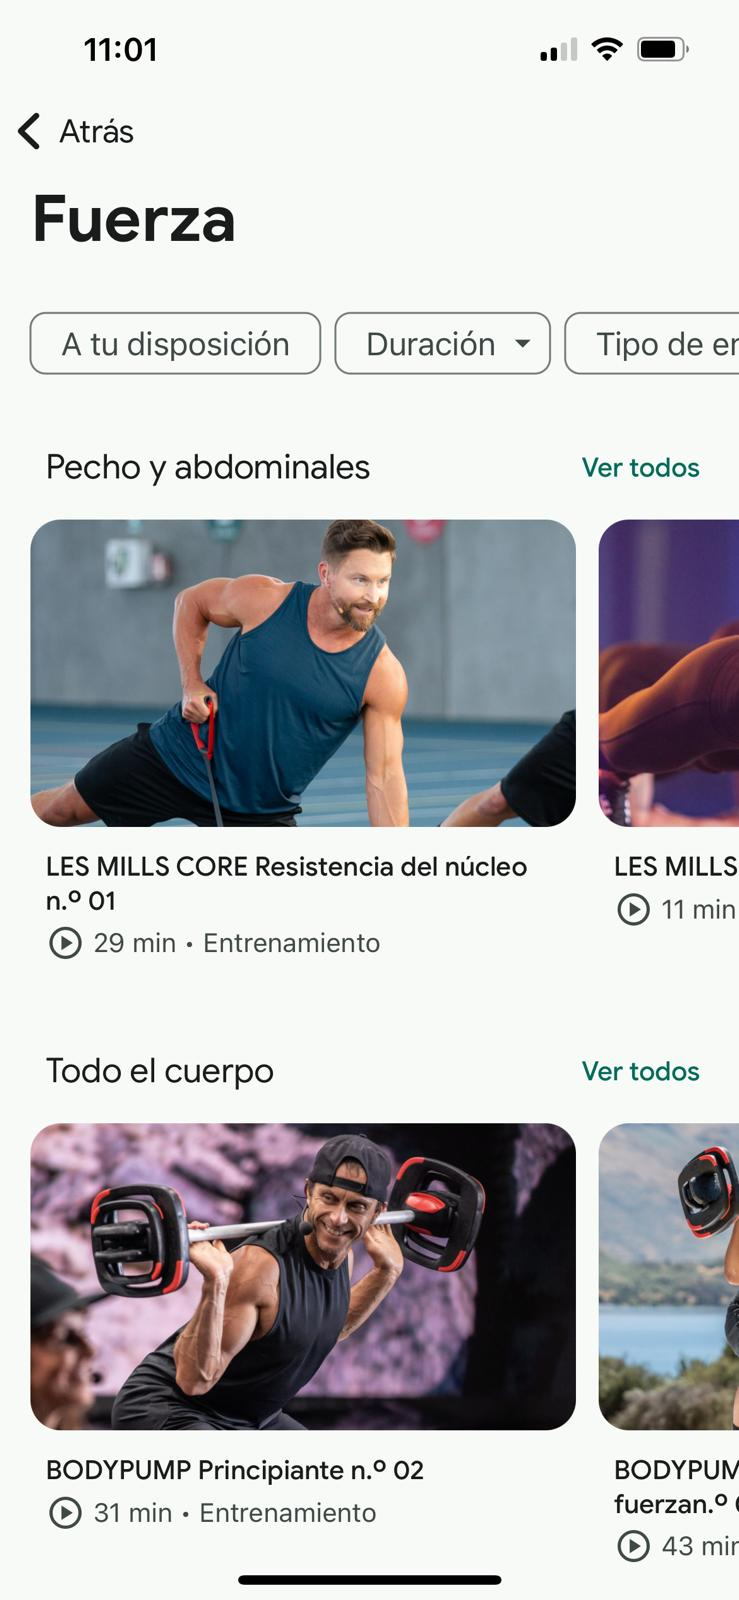
\includegraphics[width=0.5\textwidth]{fotos/fitbit.jpeg}
    \caption{Fitbit}
    \label{fig:Fitbit}
\end{figure} 
	\item \textbf{Apple Fitness+: €9.99}, en su verión gratuita nos permite guardar todas las variables permitidas con un smartwatch, las registra y va aconsejando, salta un aviso si detecta que tienes estrés, realizas poco movimiento o tienes pulsaciones anormales. En la versión de pago añade los entrenamientos, pero vuelve a la misma problemática, son entrenamientos prefijados y no permite guardar el rendimiento del usuario. (\cite{apple_fitness_plus})
\begin{figure}[H]
   \centering
    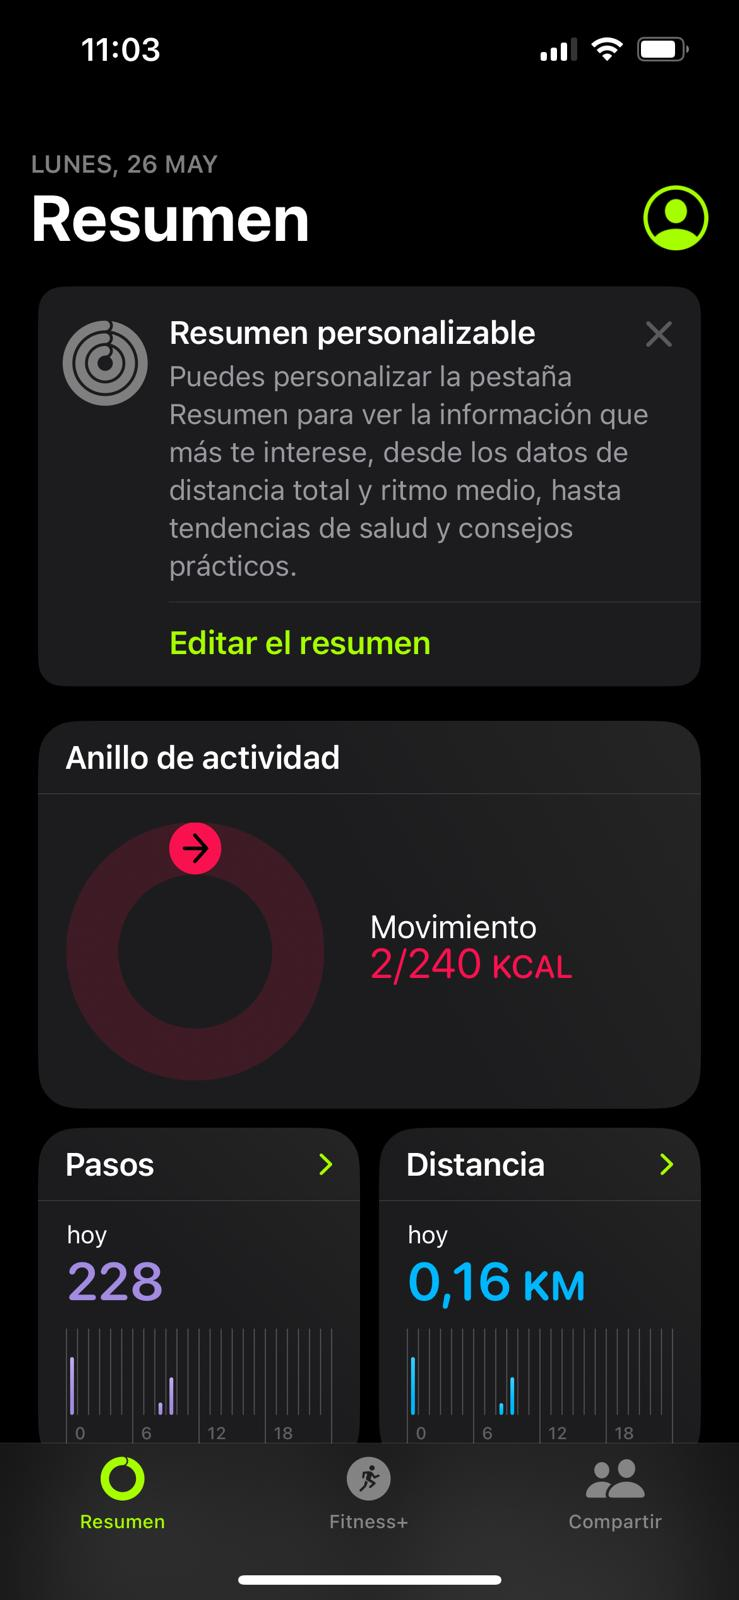
\includegraphics[width=0.5\textwidth]{fotos/fitness.jpeg}
    \caption{Apple fitness}
    \label{fig:Apple fitness}
\end{figure} 
	\item \textbf{Strava Premium: €5.99}, es una app más enfocada a running, pero permite medir variables relacionadas con este tipo de entrenamientos, kilómetros recorridos, rítmo, ruta recorrida, tiempo, etc. Es muy completa solo para ese tipo de entrenamientos. (\cite{strava})
\begin{figure}[H]
   \centering
    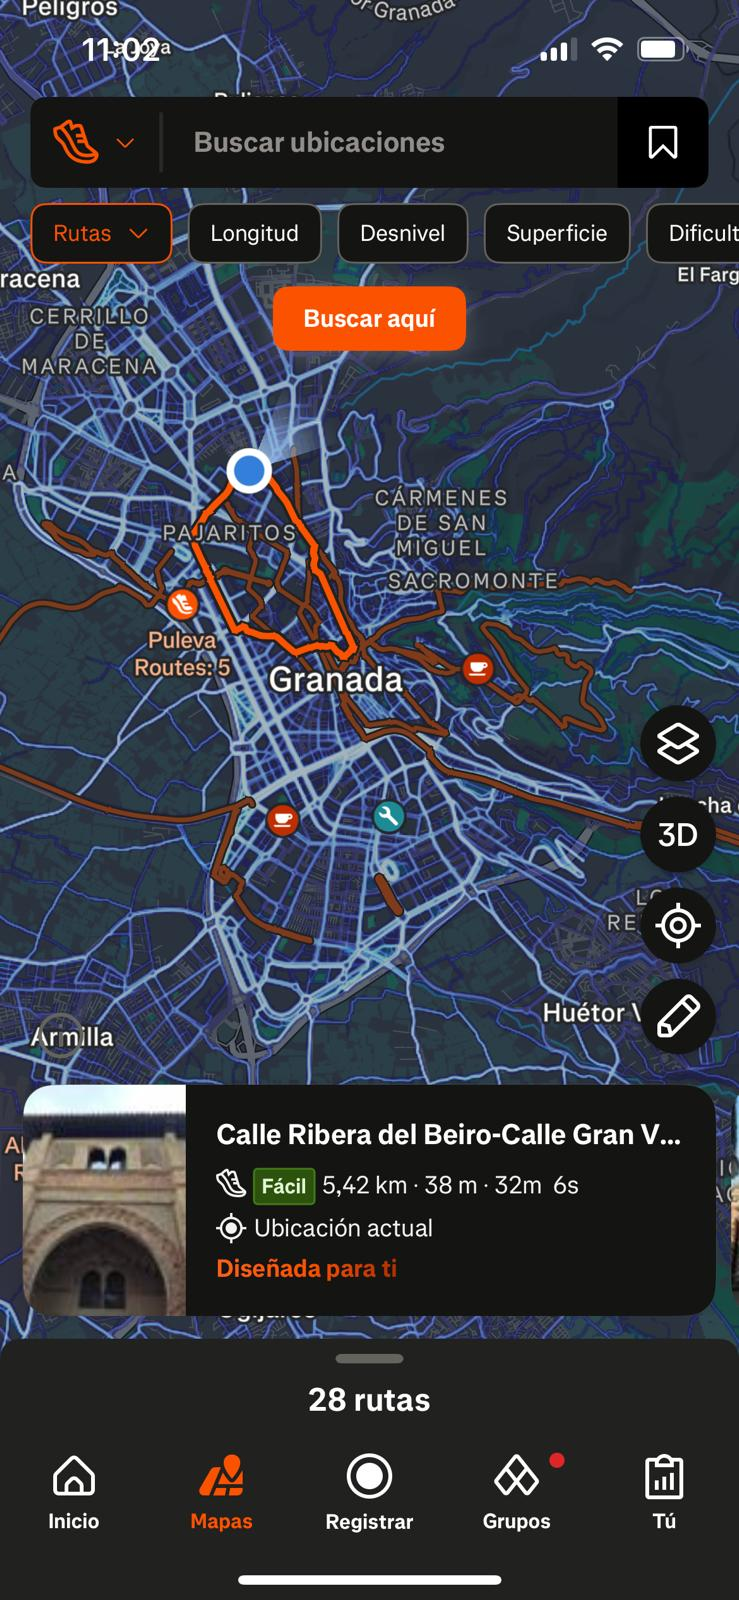
\includegraphics[width=0.5\textwidth]{fotos/strava.jpeg}
    \caption{Strava}
    \label{fig:Strava}
\end{figure} 
	\item \textbf{Whoop: €28}, de las aplicaciones esta es de lejos la más completa, permite medir estrés, cansancio del usuario, calidad del entrenamiento, calidad de sueño, recuperación y edad de tu cuerpo según tus constantes. Además, incluye una IA especializada para chatear y recibir consejos, etc. Sin embargo, es la que tiene la mensualidad más cara y solo funciona con un reloj de su marca, es decir, el usuario esta obligado a comprar ese reloj si quiere usar dicha app, el reloj en concreto vale 200€ mínimo. (\cite{whoop})
\begin{figure}[H]
   \centering
    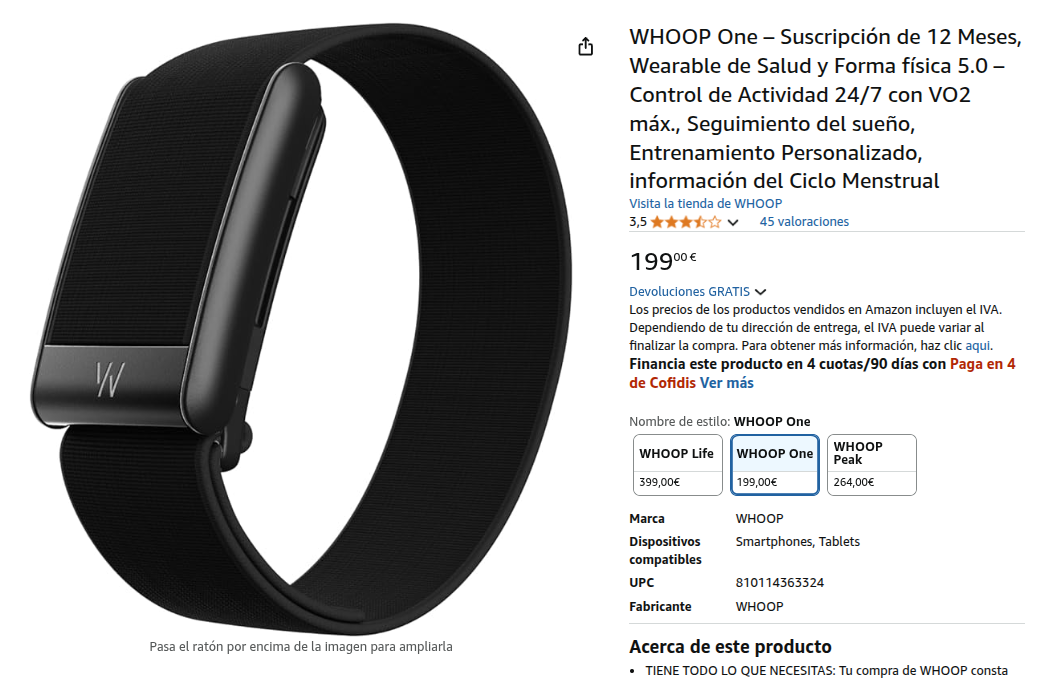
\includegraphics[width=0.5\textwidth]{fotos/Pulsera whoop.png}
    \caption{Pulsera whoop}
    \label{fig:Pulsera whoop}
\end{figure} 
\end{itemize}

Es verdad que algunas aplicaciones tienen versión gratuita, pero no ofrecen la totalidad de sus funcionalidades, de hecho, estas versiones suelen ser extremadamente limitadas. Otras aplicaciones sí que son gratuitas, pero te obligan a usar un smartwatch de la marca, por ejemplo, la app Garmin Connect requiere comprar un reloj Garmin cuyo precio no baja de los 300€.

Para clarificar las diferencias con el resto de apps del mercado:

\begin{landscape}
\begin{figure}[H]
   \centering
    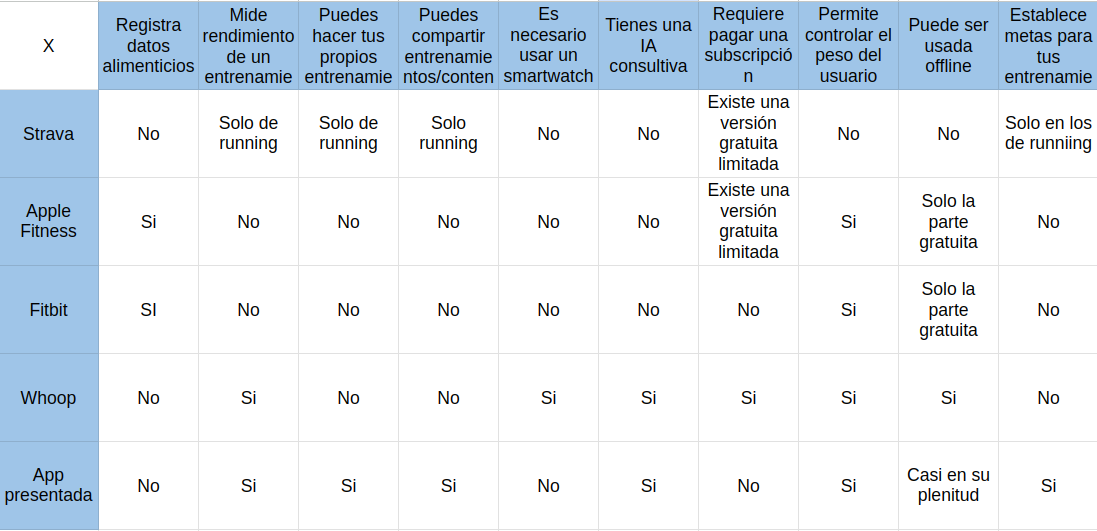
\includegraphics[width=1.65\textwidth]{tablas/tabla.png}
    \caption{Tabla comparativa de aplicaciones similares}
    \label{fig:Tabla comparativa}
\end{figure} 
\end{landscape}

\section{Metodologías potenciales a aplicar}

Existen muchas formas de desarrollar software con sus respectivas ventajas, desventajas y forma de trabajar:

\begin{itemize}
	\item \textbf{Cascada:} Es una forma de desarrollar de las más clásicas y lineales. Se hace una secuencia de fases de desarrollo, las cuales suelen ser diseño requisitos, diseño, implementación, pruebas, implementación y mantenimiento. Es una metodología fácil de entender y aplicar, eficaz para plazos de entrega estrictos. Sin embargo, no es flexible, y si se encuentran fallos en la planificación o alguna de las fases, no hay mucho tiempo de reacción.
	\item \textbf{Desarrollo Ágil:} En lugar de una secuencia rígida de fases, se promuebe la flexibilidad, ya que se combina con reuniones con el cliente para obtener feedback del software funcional desarrollado entregado en dichas reuniones(no es un prototipo ya que solo es una demostración, no se le entrega para su uso durante el desarrollo), permitiendo corregir errores de planificación o en el propio software durante el desarrollo, sin perder mucho tiempo. Es necesario un buen feedback del cliente.
	\item \textbf{Lean Software Development: } Se basa en la idea de descartar todo aquello que no aporte valor para el cliente y quitarle importancia al desarrollo para ganar calidad y sostenibilidad en el tiempo al software. Esto se refleja en que primero se hace una investigación a fondo de todas las herramientas posibles a usar, su consecuente aprendizaje y en lo más tardio de todo esta la elección de que herramientos usar. Una vez hecha la elección, ya se puede empezar con el desarrollo.
	\item \textbf{V Model: } Es como el método cascada, pero antes de pasar a la siguiente fase se realizan las pruebas de la actual y no se procede hasta que estas estén válidas. Sigue teniendo las mismas desventajas que el modelo de cascada, pero es ideal para proyectos en los que es necesaria una alta calidad.
	\item \textbf{Modelo en espiral: } En cada fase se realiza planificación, diseño, desarrollo y evaluación de riesgos. Es muy flexible y esta analizando constantemente los riesgos.
\end{itemize}

Todas estas metodologías vienen explicadas en con sus ventajas y desventajas en \cite{anwer2017sdlc} (Cascada, V-model y desarrollo ágil), \cite{poppendieck2012lean} (Lean Software Development) y \cite{boehm1988spiral} (Modelo en espiral)

\section{Tecnologías potenciales para usar}

Para hablar de las tecnologías a emplear, se separará en 3 partes importantes en un desarrollo como el que se va a abordar: la base de datos, el backend y el frontend.

\subsection{Base de datos}

En este punto vamos a hablar de las ventajas y desventajas entre usar BDs relacionales y no relacionales, así como las herramientas a emplear en cada una para desarrollar estos servicios.

\textbf{Relacionales:} Las bases de datos relacionales o SQL, como bien sabemos nos permiten guardar datos de una manera bien definida y estructurada, permitiendo asegurar la integridad de la información almacenada. Son muy buena opción, si se prefiere una escalabilidad vertical, es decir, aumentar la capacidad de procesamiento del servidor que va a albergar la BD. Algunas de los SGBDS existentes en la actualidad son:

\begin{itemize}
	\item MySQL
	\item MariaDB
	\item Oracle Database
	\item SQL server(Microsoft)
	\item PostgreSQL
\end{itemize}

\textbf{No relacionales:} También llamadas NoSQL, sirven para trabajar con estructuras de datos semidefinidas o no definidas. Esto quiere decir que no siguen un esquema rígido, lo cuál puede complicar consultas complejas, pero permiten una gran escalabilidad horizontal, permiten añadir más servidores para que operen con la misma base de datos, por tanto aumentar el número de peticiones que puede atender. Cabe decir que dentro de este tipo de bases de datos existen varios subtipos, cada uno especializado en una cualidad, al final se incluye una tabla comparativa:

\begin{itemize}
	\item Documentales(p.e. MongoDB): guardan los datos en un JSON
	\item Columnares(p.e. Cassandra): los datos no se guardan en filas, sino en columnas ,ideal para tratar grandes volumenes de datos por columnas
	\item Clave-Valor(p.e. DynamoDB): acceso rápido a los datos
	\item Graficas(p.e. Amazon Neptune): para tratar relaciones complejas
\end{itemize}

\begin{figure}[H]
   \centering
    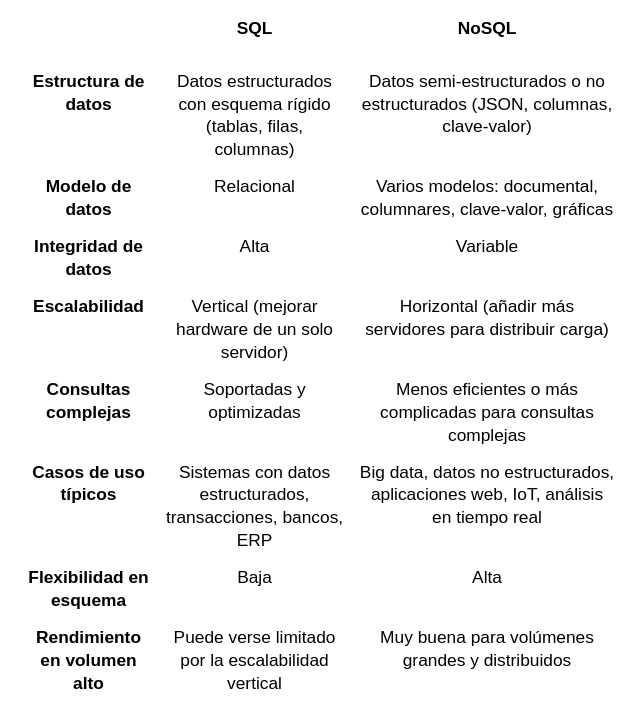
\includegraphics[width=\textwidth]{tablas/BDS.png}
    \caption{Tabla comparativa tipos de bases de datos}
    \label{fig:Tabla BDS}
\end{figure} 

\subsection{Backend}
En el desarrollo del backend exiten varios frameworks que nos van a permitir un desarrollo rápido, eficaz y de calidad. Nuetro backend se va encargar principalmente de recibir y realizar peticiones de los clientes y/o consultas a la BD. Para ello se han investigado las siguientes herramientas:
\begin{itemize}
	\item Express.js(p.e. Node.js): muy escalable y alto rendimiento
	\item Django(p.e. Python): ideal para sistemas a gran escala
	\item Ruby on rails: el mejor en velociad de desarrollo
\end{itemize}
Existen más frameworks, pero hemos decidido investigar solo sobre aquellos que me permitan un desarrollo más ágil, el resto de herramientas como Spring Boot(Java) o Laravel(PHP), también son buenas herramientas, pero tenemos más familiaridad con algunas de las herramientas anteriores, a continuación se muesra una tabla comparativa entre ellas.

\newpage

\begin{figure}[H]
   \centering
    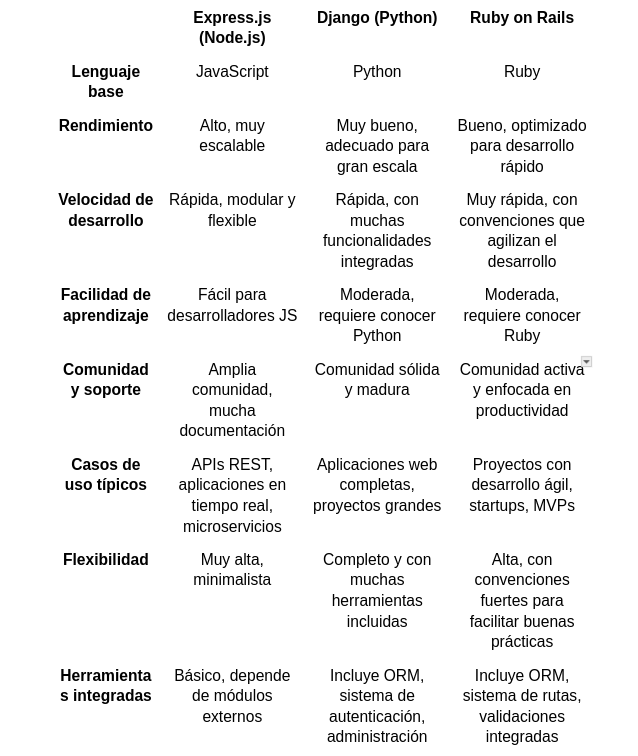
\includegraphics[width=\textwidth]{tablas/Backend.png}
    \caption{Tabla comparativa frameworks para el backend}
    \label{fig:Tabla backend}
\end{figure}

\subsection{Frontend}

Como se dijo en la introducción, uno de los objetivos es que el software sea multiplataforma, así que se investigará sobre frameworks que me permitan esa capacidad, después se muestra una tabla comparatva:

\begin{itemize}
	\item Flutter(lenguaje Dart): de las manos de Google, esta herramienta permite un desarrollo rápido ya que nos permite el hot reload y no tener que recompilar la app cada vez que haya un cambio. También es muy personalizable en lo que respecta a la UI.
	\item React Native(lenguaje JavaScript): es un framework que extiende React, permitiendo hacer sentir aplicaciones en js como si fueran nativas.
	\item Xamarín(Lenguajes C\#): de Microsoft, esta herramienta es ideal para desarrolladores familiarizados con C\# y .NET, también es idóneo para el alto rendimiento y acceso a HW nativo.
\end{itemize}

\begin{figure}[H]
   \centering
    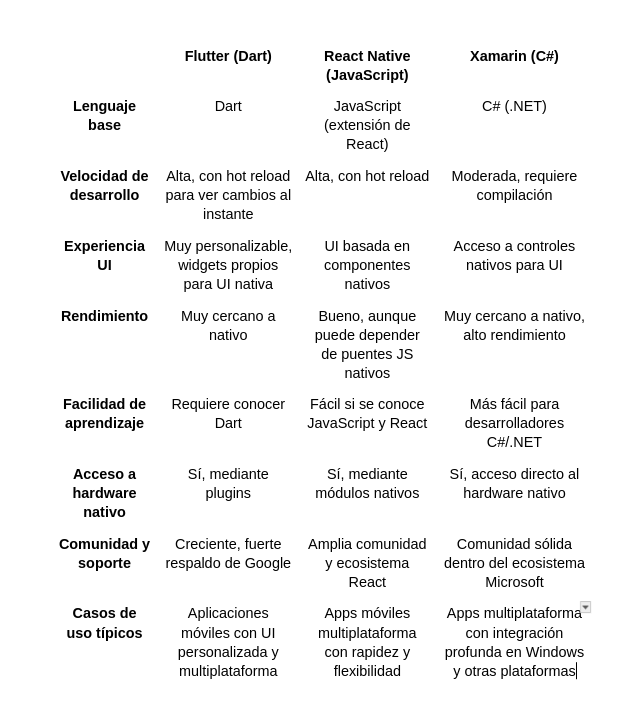
\includegraphics[width=\textwidth]{tablas/Frontend.png}
    \caption{Tabla comparativa frameworks para el frontend}
    \label{fig:Tabla frontend}
\end{figure} 